% Chapter 2

\chapter{Path algorithms} % Main chapter title

\label{Chapter6} % For referencing the chapter elsewhere, use \ref{Chapter1} 

\lhead{Chapter 6. \emph{Path algorithms}} % This is for the header on each page - perhaps a shortened title

%----------------------------------------------------------------------------------------
Finding the shortest path is one of the main problems in graph theory. It is a problem of finding a path between two nodes, where the sum of edge weights must be minimized. Graph can be undirected, directed or mixed.
\par The analogy with road maps can be clearly seen, where nodes correspond to intersections and road segments to edges on the graph. To properly represent one way streets we use directed graph. The weight of each edge can be interpreted as a length of each road segment.
\par There are numerous algorithms that are able to found the shortest path. After initial research we narrowed the possible algorithms to:
\begin{itemize}
\item Dijkstra's algorithm
\item A* search algorithm
\item Bellman - Ford algorithm
\item Floyd - Warshall algorithm
\end{itemize}
From the user requirement analysis (segment \ref{user_req}) we were able to identify the three main user requests involving path algorithms:
\begin{itemize}
\item Find shortest path from point A to B (by foot or by car);
\item Find the shortest way to all POIs of a certain category in a radius from point A (by foot or by car);
\item Construct an itinerary from point A to B with visiting POIs in between (with max distance limit);
\end{itemize}

From identified requirements, we can see that all of our path finding problems are actually problems of finding paths between points A and B. This are so-called \textbf{single-pair shortest path problems}. Analysing the algorithms listed above we determined that:
\begin{itemize}
\item Floyd - Warshall algorithm finds shortest paths between every pair of nodes in the graph;
\item Dijkstra and Bellman - Ford algorithms find the shortest paths between source node and all other nodes on the graph (Bellman - Ford also permits negative weights);
\item A* algorithm finds the shortest path between the source and target node. 
\end{itemize}

All of the above algorithms encapsulate the result which we need, but differing in how many unnecessary paths are also calculated. This subsequently mean longer calculation times, which we want to avoid. For this reasons we chose \textbf{A* algorithm} for our path finding problems.

\section{A* algorithm}
A* algorithm is one of the most popular path finding algorithms. Its ability to combine the benefits of Dijkstra's algorithm (favouring nodes close to the start node) and Best-First-Search algorithms (favouring nodes close to the target node) makes it efficient and accurate. 
\subsection{Process}
Algorithm works by traversing the graph node by node till it reaches the end node. At every step, node with the lowest cost $(f(x))$ is selected. Calculation of the cost and selection of the node is what sets A* algorithm apart from other greedy best-first search algorithms. Cost is calculated as a weighted sum of:
\begin{itemize}
\item $g(n) - $\textit{exact cost} of the path from the starting point,
\item $h(n) - $\textit{heuristic estimated cost}.
\end{itemize}
Heuristics are used to control the A*'s behaviour. If $h(n)=0$ only distance from the start node matters and we have normal Dijkstra algorithm. Because we do not know the real distance from observed node to the end target, as we haven't traversed it yet, we have to estimate it. It is important not to overestimate the distance, as this can cause the algorithm not to found the shortest path. We decided to use the air distance as a heuristic, as this guarantees that the actual distance will be equal or greater than that, so we will never over-estimate it.

\section{Road snapping}
As described in the previous section A* algorithm enables us to find the shortest path between two nodes in a graph. This enforces the restriction of searching only on the locations of the nodes. This is a huge limitation, as on some parts of the map users defined point can be located far away from the closest node. To overcome this restriction we implemented \textbf{a road snapping function}.
\par
\textbf{Road snapping function} finds the segment on which the perpendicular projection of user's point is closest to the user's point itself. We only consider the segments which are appropriate for a specific mode of transport. Calculation of the perpendicular projection of a point on the segment is done using vectors and dot product between them. Algorithm used is described on website (\cite{notmagi}). It is worth mentioning that if the perpendicular projection of the point is outside of the interval between both nodes, it snaps to the closer border node. This can be seen on figure\ref{fig:db_snap} (left and right).

\begin{figure}[h]
\centering
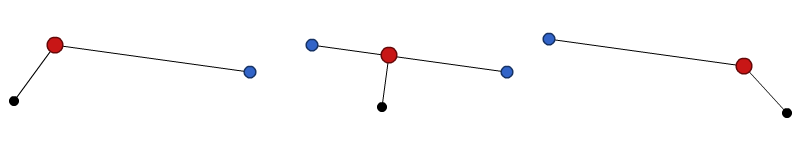
\includegraphics[width=0.9\linewidth]{../pictures/snap_points.png}
\caption{Snapping user point to border nodes (left,right) and snapping to perpendicular point where possible}
\label{fig:db_snap}
\end{figure}

With perpendicular projected point we create a \textit{new mock node} which represents the start point of our search on the road. We connect this new node with the end nodes of the closest segment, making it possible to use it in A* algorithm. We repeat the same steps for the end point. After the search we remove all the nodes and edges we additional added, reverting back the graph to the same state as before the search.

\subsection{Implementation in C++}
Road snapping function requires an extremely time consuming operation of finding close segments. One possible solution would be to actually calculate the perpendicular projections on every WaySegment in the database and then among them find the smallest. This would mean thousands of unnecessary calculations. Instead we used rtree data structure containing all the WaySegments implemented in \textit{Database class}. With this we were able to quickly find WaySegments whose bounding boxes intersect with our point. To compensate for areas, where roads are closely together, we implemented the search in small increasing steps. We start the with a small neighbourhood and gradually increase it, until we find any intersecting WaySegments. This approach reduces the calculations of perpendicular projections from thousand to just a couple. The diagram of the proces is shown in the figure \ref{fig:closestWaySegment}

\begin{figure}[h]
\centering
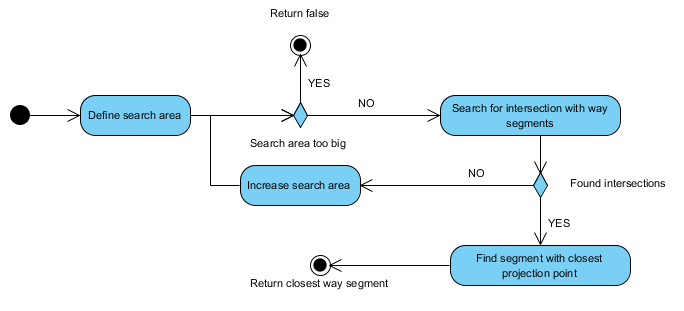
\includegraphics[width=0.7\linewidth]{../pictures/act_diagram_closest_way.png}
\caption{Diagram of finding the closest WaySegment}
\label{fig:closestWaySegment}
\end{figure}

\subsection{Implementation in Matlab}
Unfortunately Matlab does not have similar data structures capable of spatial filtering. To get the same end result we calculated the projection points on all the points and find the one with the minimal distance. To speed up the process of calculation we put the data in vectors and vectorize (\cite{matlab1}) the code for calculation. The speed of the calculation turned out to be sufficient.

\section{Shortest path A $->$ B}
This algorithm finds the shortest path between users defined points A and B on the roads that permit mode of transport selected by the user. With the usage of the road snapping functionality we can provide the user complete freedom in selecting the points anywhere on the map. The inputs to the algorithm are:
\begin{itemize}
\item Location of the start point
\item Location of the end point
\item Mode of transport
\end{itemize}
After finding the closest segments for start and end and adding mock nodes we can use A* algorithm to find the shortest path. The result of the algorithm is an object Path containing one PathSegment corresponding to WaySegments on the way from point A to B. If path does not exist we return an empty Path. The whole process is schematically shown on figure \ref{fig:ab_activity}.
\begin{figure}[h]
\centering
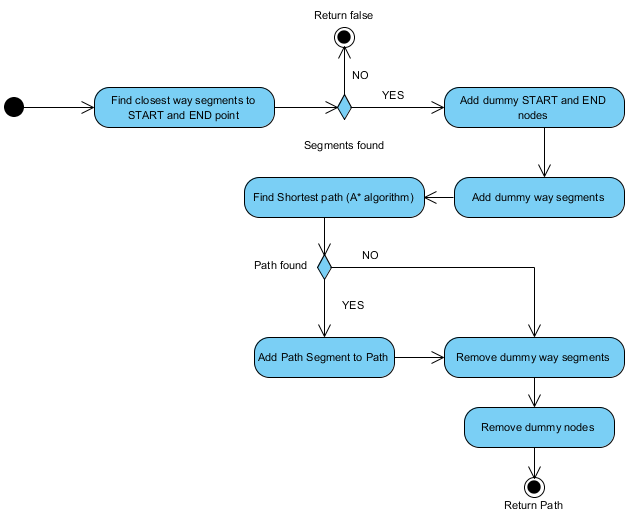
\includegraphics[width=0.8\linewidth]{../pictures/shortest_path_ab_activity.png}
\caption{Activity diagram of finding the shortest path between point A and B}
\label{fig:ab_activity}
\end{figure}

\subsection{Implementation}
The implementation details for both applications (C++ and Matlab) have been already described in specific methods of A* and road snapping. Other things are just sequence of if sentences that do not need special explanation.
Figures \ref{fig:ab_result_cpp} and \ref{fig:ab_result_matlab} shows the end result of the search as seen by the user.
\begin{figure}[h]
\centering
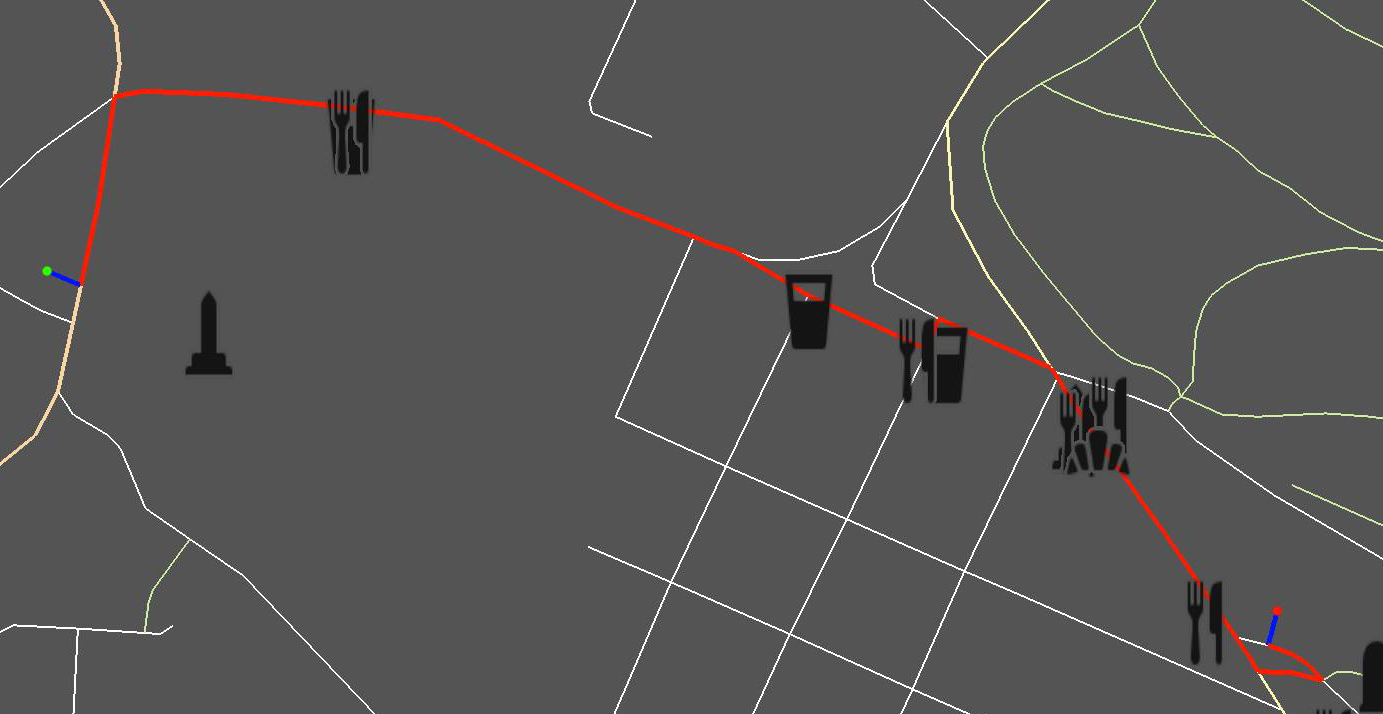
\includegraphics[width=0.8\linewidth]{../pictures/search_ab_result.jpg}
\caption{Result of the search for the shortest path as seen by the user in C++}
\label{fig:ab_result_cpp}
\end{figure}
\begin{figure}[h]
\centering
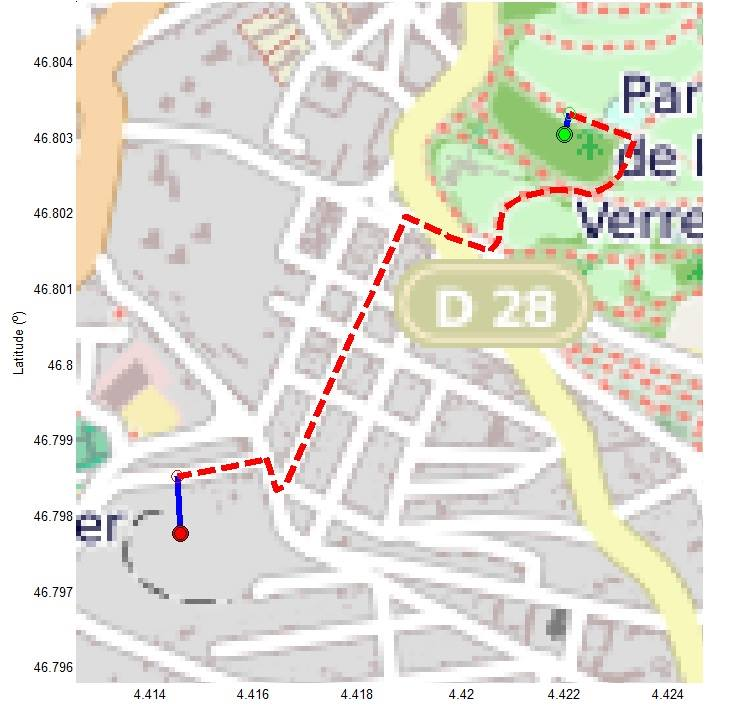
\includegraphics[width=0.6\linewidth]{../pictures/search_ab_matlab.jpg}
\caption{Result of the search for the shortest path as seen by the user in Matlab}
\label{fig:ab_result_matlab}
\end{figure}

\section{Radius search}
Radius search algorithm finds all the possible paths from user defined point A to all the points of interest (POIs) of a user specified category in some radius. The inputs to the algorithm are:
\begin{itemize}
\item Location of the start point
\item Category of POIs
\item Max distance of the path
\item Mode of transport
\end{itemize}
After finding the closest WaySegment to the start point, we go through all the POIs. For each of them we find the closest WaySegment and check the air distance between start and POI point. If the distance is bigger than the longest permitted path, we immediately discard the POI, because there is shorter way possible than that. Otherwise we try to find the shortest path using \textbf{Shortest path A $->$ B algorithm}. The final result of the algorithm is a bit different for both applications. In C++ we return the set of all possible paths ordered by the distance of the path, whereas in Matlab we only return the shortest path. Whole process is shown on figure \ref{fig:radius_activity}.    
 \begin{figure}[h]
 \centering
 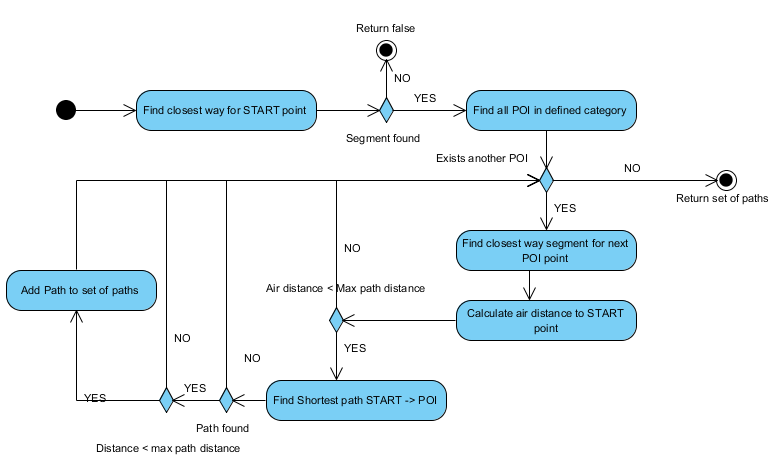
\includegraphics[width=0.8\linewidth]{../pictures/shortest_path_radius.png}
 \caption{Activity diagram of finding radius search between point A and POIs of specific categories}
 \label{fig:radius_activity}
 \end{figure}
 \subsection{Implementation in C++}
 As mentioned, data structure used to store all found paths is \textit{std::set}. We used that because our paths are unique and we want them ordered by distance. For this reason we implemented comparator that takes care of sorting the paths when they are inserted in the set. Figure \ref{fig:radius_result} shows the end result of the search as seen by the user.
 
\begin{figure}[h]
\centering
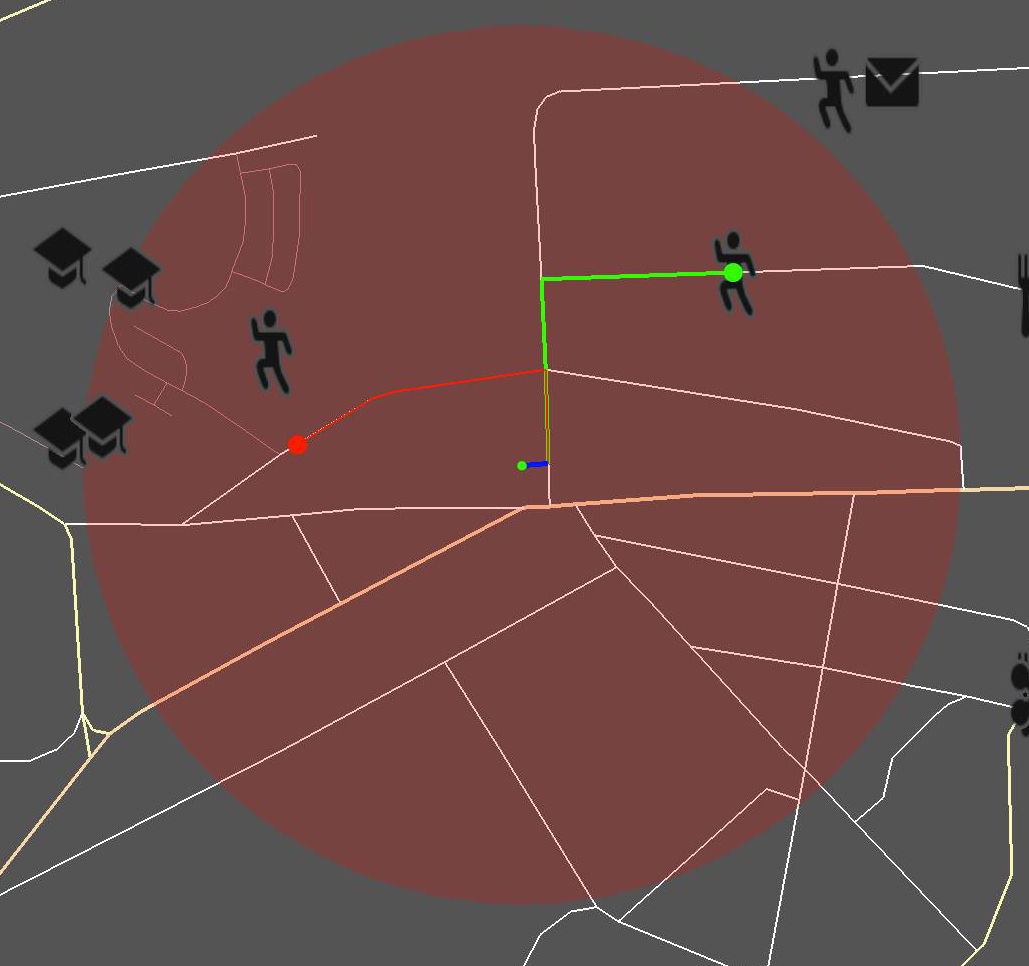
\includegraphics[width=0.8\linewidth]{../pictures/search_radius_result.jpg}
\caption{Result of the radius search as seen by the user in C++}
\label{fig:radius_result}
\end{figure}

 \subsection{Implementation in Matlab}
 In Matlab we implemented the algorithm using vectors and with the usage of vectorization. The calculations are not as efficient as in C++, but the usage of vectorization enables us to have results in sufficient amount of time. 
 
 
\section{Itinerary search}
Itinerary search algorithm constructs a path, that connects users defined start and end point and go through points of interested of a user defined categories. Algorithm finds a path that goes through one of the POI of each of the categories. The number of the categories in the list (points we want to visit) is not limited by the algorithm, but we have limited it in UI, because we have to be aware that the number of combinations increases significantly with every new category. Algorithm's inputs are:
\begin{itemize}
\item Location of the start point
\item Location of the end point
\item List of Categories of POIs we want to visit
\item Max distance of the path
\item Indication if the order of visited categories is important
\item Mode of transport
\end{itemize}
Before the start of actual path finding, we construct all possible combinations of POIs on the way. As already mentioned, for each category in the list we want to visit just one POI. We add list of points for each of the combinations to a queue which is ordered by ascending order of the sum of air distances of points on the path.
\par
Next phase is to find an actual path. We always look for the actual path of the list of points that have the smallest sum of air distance in the queue (top of the queue). If the air distance of the top element of the queue is bigger than the minimum distance found of the real path, we can stop the search, as we will not find smaller path then the one we already have. This way we do not keep looking for numerous paths which do not have any chance of being smaller, than the minimal path already found. Diagram in figure \ref{fig:itinerary_activity}] shows the process of the search. The same as in previous algorithms, if no path is found we return an empty path.
 \begin{figure}[h]
 \centering
 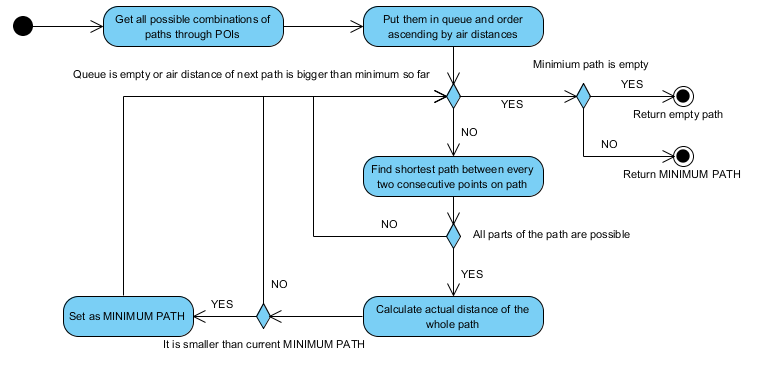
\includegraphics[width=0.7\linewidth]{../pictures/shortest_path_itinerary.png}
 \caption{Activity diagram of finding shortest path from A to B through POIs of specific categories}
 \label{fig:itinerary_activity}
 \end{figure}
 
\subsection{Implementation in C++}
Described algorithm was implemented in C++, using list data structure, to hold all the possible combinations of POIs and priority queue to sort the paths according the air distances. We used the selected data structures because they provided exactly what we needed. Priority queue because the order of our data is important and the smallest(largest) element goes out first. Figure \ref{fig:ite_result_cpp} shows the end result of the search as seen by the user.
\begin{figure}[h]
\centering
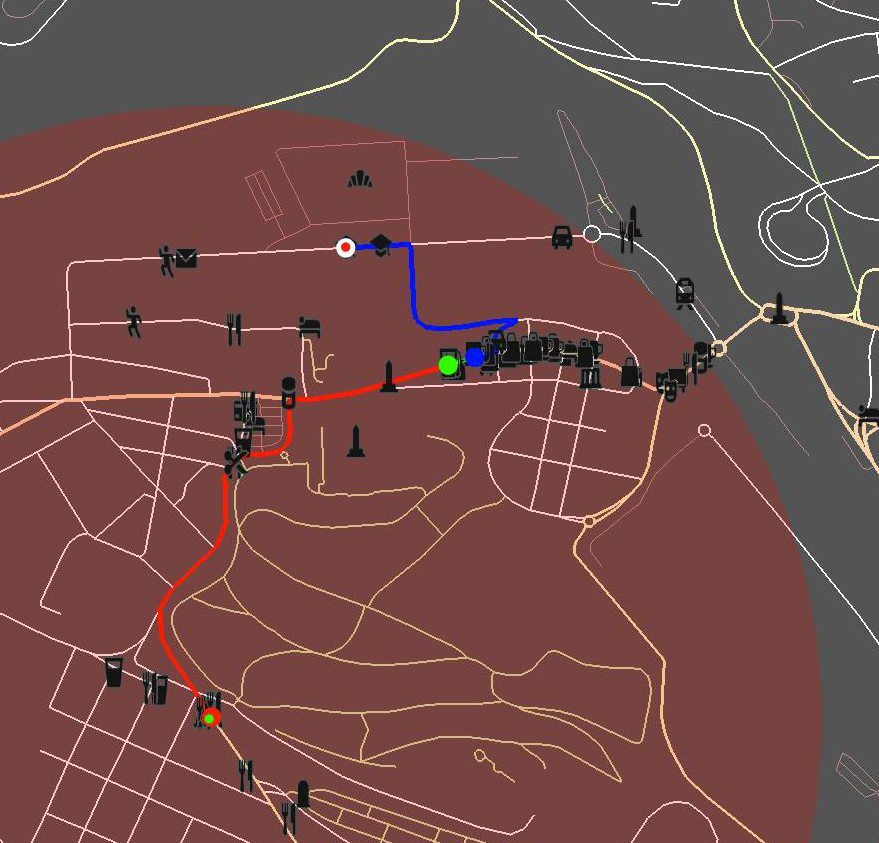
\includegraphics[width=0.8\linewidth]{../pictures/search_ite_result.jpg}
\caption{Result of the itinerary search as seen by the user in C++}
\label{fig:ite_result_cpp}
\end{figure}
\subsection{Implementation in Matlab}
In Matlab we have implemented the algorithm with only one middle category. In the calculations we take advantage of Vectorization, which significantly increases the speed of the calculations. Figure \ref{fig:ite_result_matlab} shows the end result of the search as seen by the user.   
\begin{figure}[h]
\centering
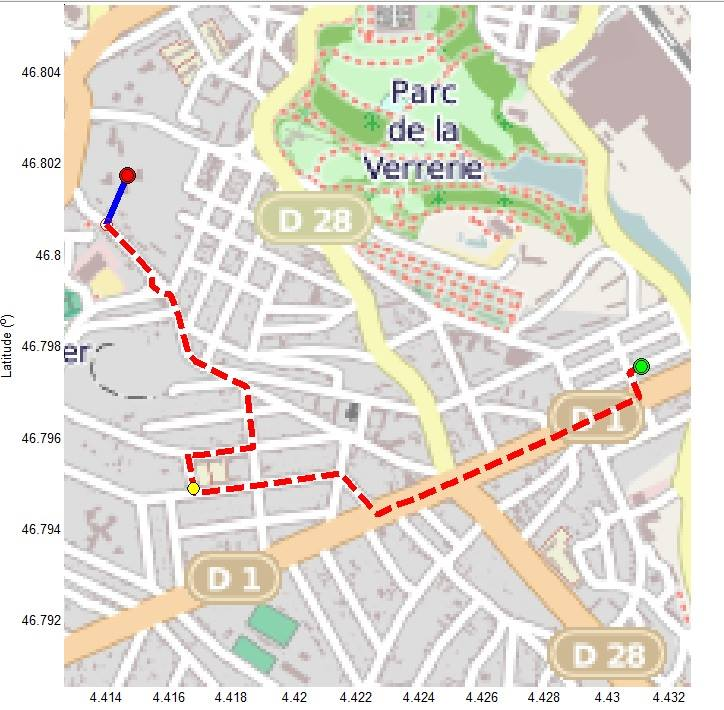
\includegraphics[width=0.6\linewidth]{../pictures/search_ite_matlab.jpg}
\caption{Result of the itinerary search as seen by the user in Matlab}
\label{fig:ite_result_matlab}
\end{figure}